\section{Navigation/Terminology}\label{navigationterminology}

\subsection{Design a file system! What are your design
goals?}\label{design-a-file-system-what-are-your-design-goals}

The design of a file system is difficult problem because there many
high-level design goals that we'd like to satisfy. An incomplete list of
ideal goals include:

\begin{itemize}
\tightlist
\item
  Reliable and robust (even with hardware failures or incomplete writes
  due to power loss)
\item
  Access (security) controls
\item
  Accounting and quotas
\item
  Indexing and search
\item
  Versioning and backup capabilities
\item
  Encryption
\item
  Automatic compression
\item
  High performance (e.g.~Caching in-memory)
\item
  Efficient use of storage de-duplication
\end{itemize}

Not all filesystems natively support all of these goals. For example,
many filesystems do not automatically compress rarely-used files

\subsection{\texorpdfstring{What are \texttt{.}, \texttt{..}, and
\texttt{...}?}{What are ., .., and ...?}}\label{what-are-.-..-and-...}

In standard unix file systems: * \texttt{.} represents the current
directory\\
* \texttt{..} represents the parent directory\\
* \texttt{...} is NOT a valid representation of any directory (this not
the grandparent directory). It \emph{could} however be the name of a
file on disk.

\subsection{What are absolute and relative
paths?}\label{what-are-absolute-and-relative-paths}

Absolute paths are paths that start from the `root node' of your
directory tree. Relative paths are paths that start from your current
position in the tree.

\subsection{What are some examples of relative and absolute
paths?}\label{what-are-some-examples-of-relative-and-absolute-paths}

If you start in your home directory (``\textasciitilde{}'' for short),
then \texttt{Desktop/cs241} would be a relative path. Its absolute path
counterpart might be something like
\texttt{/Users/{[}yourname{]}/Desktop/cs241}.

\subsection{\texorpdfstring{How do I simplify
\texttt{a/b/../c/./}?}{How do I simplify a/b/../c/./?}}\label{how-do-i-simplify-ab..c.}

Remember that \texttt{..} means `parent folder' and that \texttt{.}
means `current folder'.

Example: \texttt{a/b/../c/./} - Step 1: \texttt{cd\ a} (in a) - Step 2:
\texttt{cd\ b} (in a/b) - Step 3: \texttt{cd\ ..} (in a, because ..
represents `parent folder') - Step 4: \texttt{cd\ c} (in a/c) - Step 5:
\texttt{cd\ .} (in a/c, because . represents `current folder')

Thus, this path can be simplified to \texttt{a/c}.

\section{So what's a File System?}\label{so-whats-a-file-system}

A filesystem is how information is organized on disk. Whenever you want
to access a file, the filesystem dictates how the file is read. Here is
a sample image of a filesystem.

\begin{figure}[htbp]
\centering
\includegraphics{http://tinf2.vub.ac.be/~dvermeir/manual/uintro/disk.gif}
\caption{}
\end{figure}

Whoa that's a lot let's break it down * Superblock: This block contains
metadata about the filesystem, how large, last modified time, a journal,
number of inodes and the first inode start, number of data block and the
first data block start. * Inode: This is the the key abstraction. An
inode is a file. * Disk Blocks: These are where the data is stored. The
actual contents of the file

\subsection{How does inode store the file
contents?}\label{how-does-inode-store-the-file-contents}

\begin{figure}[htbp]
\centering
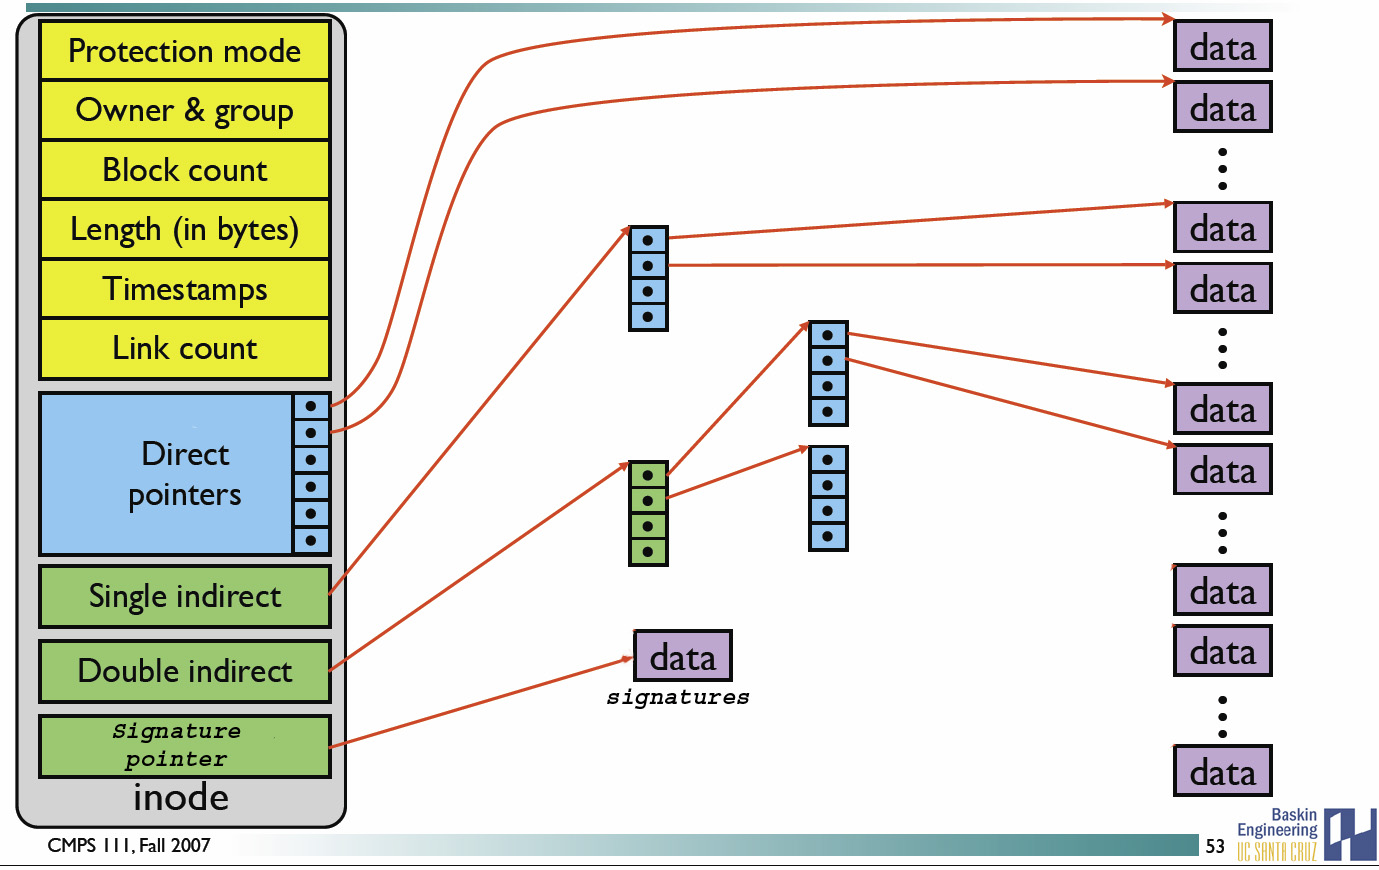
\includegraphics{https://classes.soe.ucsc.edu/cmps111/Fall08/inode_with_signatures.jpg}
\caption{}
\end{figure}

From \href{http://en.wikipedia.org/wiki/Inode}{Wikipedia}:

\begin{quote}
\emph{In a Unix-style file system, an index node, informally referred to
as an inode, is a data structure used to represent a filesystem object,
which can be one of various things including a file or a directory. Each
inode stores the attributes and disk block location(s) of the filesystem
object's data. Filesystem object attributes may include manipulation
metadata (e.g.~change, access, modify time), as well as owner and
permission data (e.g.~group-id, user-id, permissions).}
\end{quote}

To read the first few bytes of the file, follow the first direct block
pointer to the first direct block and read the first few bytes, writing
is the same process. If you want to read the entire file, keep reading
direct blocks until your size runs out (we will talk about indirect
blocks in a bit)

\begin{quote}
``All problems in computer science can be solved by another level of
indirection.'' - David Wheeler
\end{quote}

\subsection{Why make disk blocks the same size as memory
pages?}\label{why-make-disk-blocks-the-same-size-as-memory-pages}

To support virtual memory, so we can page stuff in and out of memory.

\subsection{What information do we want to store for each
file?}\label{what-information-do-we-want-to-store-for-each-file}

\begin{itemize}
\tightlist
\item
  Filename
\item
  File size
\item
  Time created, last modified, last accessed
\item
  Permissions
\item
  Filepath
\item
  Checksum
\item
  File data (inode)
\end{itemize}

\subsection{What are the traditional permissions: user -- group -- other
permissions for a
file?}\label{what-are-the-traditional-permissions-user-group-other-permissions-for-a-file}

Some common file permissions include: * 755: \texttt{rwx\ r-x\ r-x}

user: \texttt{rwx}, group: \texttt{r-x}, others: \texttt{r-x}

User can read, write and execute. Group and others can only read and
execute. * 644: \texttt{rw-\ r-\/-\ r-\/-}

user: \texttt{rw-}, group: \texttt{r-\/-}, others: \texttt{r-\/-}

User can read and write. Group and others can only read.

\subsection{What are the the 3 permission bits for a regular file for
each
role?}\label{what-are-the-the-3-permission-bits-for-a-regular-file-for-each-role}

\begin{itemize}
\tightlist
\item
  Read (most significant bit)\\
\item
  Write (2nd bit)\\
\item
  Execute (least significant bit)
\end{itemize}

\subsection{\texorpdfstring{What do ``644'' ``755''
mean?}{What do 644 755 mean?}}\label{what-do-644-755-mean}

These are examples of permissions in octal format (base 8). Each octal
digit corresponds to a different role (user, group, world).

We can read permissions in octal format as follows:\\
* 644 - R/W user permissions, R group permissions, R world permissions\\
* 755 - R/W/X user permissions, R/X group permissions, R/X world
permissions

\subsection{How many pointers can you store in each indirection
table?}\label{how-many-pointers-can-you-store-in-each-indirection-table}

As a worked example, suppose we divide the disk into 4KB blocks and we
want to address up to 2\^{}32 blocks.

The maximum disk size is 4KB *2\^{}32 = 16TB (remember 2\^{}10 = 1024)

A disk block can store 4KB / 4B (each pointer needs to be 32 bits) =
1024 pointers. Each pointer refers to a 4KB disk block - so you can
refer up to 1024*4KB = 4MB of data

For the same disk configuration, a double indirect block stores 1024
pointers to 1024 indirection tables. Thus a double-indirect block can
refer up to 1024 * 4MB = 4GB of data.

Similarly, a triple indirect block can refer up to 4TB of data.

Big idea: Forget names of files: The `inode' is the file.

It is common to think of the file name as the `actual' file. It's not!
Instead consider the inode as the file. The inode holds the
meta-information (last accessed, ownership, size) and points to the disk
blocks used to hold the file contents.

\subsection{So\ldots{} How do we implement a
directory?}\label{so-how-do-we-implement-a-directory}

A directory is just a mapping of names to inode numbers. POSIX provides
a small set of functions to read the filename and inode number for each
entry (see below)

Let's think about what it looks like in the actual file system.
Theoretically, directories are just like actual files. The disk blocks
will contain \emph{directory entries} or \emph{dirents}. What that means
is that our disk block can look like this

\textbar{} inode\_num \textbar{} name \textbar{}
\textbar{}-----------\textbar{}------\textbar{} \textbar{} 2043567
\textbar{} hi.txt \textbar{} \ldots{}

Each directory entry could either be a fixed size, or a variable
c-string. It depends on how the particular filesystem implements it at
the lower level.

\subsection{How can I find the inode number of a
file?}\label{how-can-i-find-the-inode-number-of-a-file}

From a shell, use \texttt{ls} with the \texttt{-i} option

\begin{verbatim}
$ ls -i
12983989 dirlist.c      12984068 sandwich.c
\end{verbatim}

From C, call one of the stat functions (introduced below).

\subsection{How do I find out meta-information about a file (or
directory)?}\label{how-do-i-find-out-meta-information-about-a-file-or-directory}

Use the stat calls. For example, to find out when my `notes.txt' file
was last accessed -

\begin{Shaded}
\begin{Highlighting}[]
   \KeywordTok{struct} \NormalTok{stat s;}
   \NormalTok{stat(}\StringTok{"notes.txt"}\NormalTok{, &s);}
   \NormalTok{printf(}\StringTok{"Last accessed %s"}\NormalTok{, ctime(&s.st_atime));}
\end{Highlighting}
\end{Shaded}

There are actually three versions of \texttt{stat};

\begin{Shaded}
\begin{Highlighting}[]
       \DataTypeTok{int} \NormalTok{stat(}\DataTypeTok{const} \DataTypeTok{char} \NormalTok{*path, }\KeywordTok{struct} \NormalTok{stat *buf);}
       \DataTypeTok{int} \NormalTok{fstat(}\DataTypeTok{int} \NormalTok{fd, }\KeywordTok{struct} \NormalTok{stat *buf);}
       \DataTypeTok{int} \NormalTok{lstat(}\DataTypeTok{const} \DataTypeTok{char} \NormalTok{*path, }\KeywordTok{struct} \NormalTok{stat *buf);}
\end{Highlighting}
\end{Shaded}

For example you can use \texttt{fstat} to find out the meta-information
about a file if you already have an file descriptor associated with that
file

\begin{Shaded}
\begin{Highlighting}[]
   \NormalTok{FILE *file = fopen(}\StringTok{"notes.txt"}\NormalTok{, }\StringTok{"r"}\NormalTok{);}
   \DataTypeTok{int} \NormalTok{fd = fileno(file); }\CommentTok{/* Just for fun - extract the file descriptor from a C FILE struct */}
   \KeywordTok{struct} \NormalTok{stat s;}
   \NormalTok{fstat(fd, & s);}
   \NormalTok{printf(}\StringTok{"Last accessed %s"}\NormalTok{, ctime(&s.st_atime));}
\end{Highlighting}
\end{Shaded}

The third call `lstat' we will discuss when we introduce symbolic links.

In addition to access,creation, and modified times, the stat structure
includes the inode number, length of the file and owner information.

\begin{Shaded}
\begin{Highlighting}[]
\KeywordTok{struct} \NormalTok{stat \{}
               \NormalTok{dev_t     st_dev;     }\CommentTok{/* ID of device containing file */}
               \NormalTok{ino_t     st_ino;     }\CommentTok{/* inode number */}
               \NormalTok{mode_t    st_mode;    }\CommentTok{/* protection */}
               \NormalTok{nlink_t   st_nlink;   }\CommentTok{/* number of hard links */}
               \NormalTok{uid_t     st_uid;     }\CommentTok{/* user ID of owner */}
               \NormalTok{gid_t     st_gid;     }\CommentTok{/* group ID of owner */}
               \NormalTok{dev_t     st_rdev;    }\CommentTok{/* device ID (if special file) */}
               \NormalTok{off_t     st_size;    }\CommentTok{/* total size, in bytes */}
               \NormalTok{blksize_t st_blksize; }\CommentTok{/* blocksize for file system I/O */}
               \NormalTok{blkcnt_t  st_blocks;  }\CommentTok{/* number of 512B blocks allocated */}
               \NormalTok{time_t    st_atime;   }\CommentTok{/* time of last access */}
               \NormalTok{time_t    st_mtime;   }\CommentTok{/* time of last modification */}
               \NormalTok{time_t    st_ctime;   }\CommentTok{/* time of last status change */}
           \NormalTok{\};}
\end{Highlighting}
\end{Shaded}

\subsection{How do I list the contents of a directory
?}\label{how-do-i-list-the-contents-of-a-directory}

Let's write our own version of `ls' to list the contents of a directory.

\begin{Shaded}
\begin{Highlighting}[]
\OtherTok{#include <stdio.h>}
\OtherTok{#include <dirent.h>}
\OtherTok{#include <stdlib.h>}
\DataTypeTok{int} \NormalTok{main(}\DataTypeTok{int} \NormalTok{argc, }\DataTypeTok{char} \NormalTok{**argv) \{}
    \KeywordTok{if}\NormalTok{(argc == }\DecValTok{1}\NormalTok{) \{}
        \NormalTok{printf(}\StringTok{"Usage: %s [directory]}\CharTok{\textbackslash{}n}\StringTok{"}\NormalTok{, *argv);}
        \NormalTok{exit(}\DecValTok{0}\NormalTok{);}
    \NormalTok{\}}
    \KeywordTok{struct} \NormalTok{dirent *dp;}
    \NormalTok{DIR *dirp = opendir(argv[}\DecValTok{1}\NormalTok{]);}
    \KeywordTok{while} \NormalTok{((dp = readdir(dirp)) != NULL) \{}
        \NormalTok{puts(dp->d_name);}
    \NormalTok{\}}

    \NormalTok{closedir(dirp);}
    \KeywordTok{return} \DecValTok{0}\NormalTok{;}
\NormalTok{\}}
\end{Highlighting}
\end{Shaded}

\subsection{How do I read the contents of a
directory?}\label{how-do-i-read-the-contents-of-a-directory}

Ans: Use opendir readdir closedir For example, here's a very simple
implementation of `ls' to list the contents of a directory.

\begin{Shaded}
\begin{Highlighting}[]
\OtherTok{#include <stdio.h>}
\OtherTok{#include <dirent.h>}
\OtherTok{#include <stdlib.h>}
\DataTypeTok{int} \NormalTok{main(}\DataTypeTok{int} \NormalTok{argc, }\DataTypeTok{char} \NormalTok{**argv) \{}
    \KeywordTok{if}\NormalTok{(argc ==}\DecValTok{1}\NormalTok{) \{}
        \NormalTok{printf(}\StringTok{"Usage: %s [directory]}\CharTok{\textbackslash{}n}\StringTok{"}\NormalTok{, *argv);}
        \NormalTok{exit(}\DecValTok{0}\NormalTok{);}
    \NormalTok{\}}
    \KeywordTok{struct} \NormalTok{dirent *dp;}
    \NormalTok{DIR *dirp = opendir(argv[}\DecValTok{1}\NormalTok{]);}
    \KeywordTok{while} \NormalTok{((dp = readdir(dirp)) != NULL) \{}
        \NormalTok{printf(}\StringTok{"%s %lu}\CharTok{\textbackslash{}n}\StringTok{"}\NormalTok{, dp-> d_name, (}\DataTypeTok{unsigned} \DataTypeTok{long}\NormalTok{)dp-> d_ino );}
    \NormalTok{\}}

    \NormalTok{closedir(dirp);}
    \KeywordTok{return} \DecValTok{0}\NormalTok{;}
\NormalTok{\}}
\end{Highlighting}
\end{Shaded}

Note: after a call to fork(), either (XOR) the parent or the child can
use readdir(), rewinddir() or seekdir(). If both the parent and the
child use the above, behavior is undefined.

\subsection{How do I check to see if a file is in the current
directory?}\label{how-do-i-check-to-see-if-a-file-is-in-the-current-directory}

For example, to see if a particular directory includes a file (or
filename) `name', we might write the following code. (Hint: Can you spot
the bug?)

\begin{Shaded}
\begin{Highlighting}[]
\DataTypeTok{int} \NormalTok{exists(}\DataTypeTok{char} \NormalTok{*directory, }\DataTypeTok{char} \NormalTok{*name)  \{}
    \KeywordTok{struct} \NormalTok{dirent *dp;}
    \NormalTok{DIR *dirp = opendir(directory);}
    \KeywordTok{while} \NormalTok{((dp = readdir(dirp)) != NULL) \{}
        \NormalTok{puts(dp->d_name);}
        \KeywordTok{if} \NormalTok{(!strcmp(dp->d_name, name)) \{}
        \KeywordTok{return} \DecValTok{1}\NormalTok{; }\CommentTok{/* Found */}
        \NormalTok{\}}
    \NormalTok{\}}
    \NormalTok{closedir(dirp);}
    \KeywordTok{return} \DecValTok{0}\NormalTok{; }\CommentTok{/* Not Found */}
\NormalTok{\}}
\end{Highlighting}
\end{Shaded}

The above code has a subtle bug: It leaks resources! If a matching
filename is found then `closedir' is never called as part of the early
return. Any file descriptors opened, and any memory allocated, by
opendir are never released. This means eventually the process will run
out of resources and an \texttt{open} or \texttt{opendir} call will
fail.

The fix is to ensure we free up resources in every possible code-path.
In the above code this means calling \texttt{closedir} before
\texttt{return\ 1}. Forgetting to release resources is a common C
programming bug because there is no support in the C lanaguage to ensure
resources are always released with all codepaths.

\subsection{What are the gotcha's of using readdir? For example to
recursively search
directories?}\label{what-are-the-gotchas-of-using-readdir-for-example-to-recursively-search-directories}

There are two main gotchas and one consideration: The \texttt{readdir}
function returns ``.'' (current directory) and ``..'' (parent
directory). If you are looking for sub-directories, you need to
explicitly exclude these directories.

For many applications it's reasonable to check the current directory
first before recursively searching sub-directories. This can be achieved
by storing the results in a linked list, or resetting the directory
struct to restart from the beginning.

One final note of caution: \texttt{readdir} is not thread-safe! For
multi-threaded searches use \texttt{readdir\_r} which requires the
caller to pass in the address of an existing dirent struct.

See the man page of readdir for more details.

\subsection{How do I determine if a directory entry is a
directory?}\label{how-do-i-determine-if-a-directory-entry-is-a-directory}

Ans: Use \texttt{S\_ISDIR} to check the mode bits stored in the stat
structure

And to check if a file is regular file use \texttt{S\_ISREG},

\begin{Shaded}
\begin{Highlighting}[]
   \KeywordTok{struct} \NormalTok{stat s;}
   \KeywordTok{if} \NormalTok{(}\DecValTok{0} \NormalTok{== stat(name, &s)) \{}
      \NormalTok{printf(}\StringTok{"%s "}\NormalTok{, name);}
      \KeywordTok{if} \NormalTok{(S_ISDIR( s.st_mode)) puts(}\StringTok{"is a directory"}\NormalTok{);}
      \KeywordTok{if} \NormalTok{(S_ISREG( s.st_mode)) puts(}\StringTok{"is a regular file"}\NormalTok{);}
   \NormalTok{\} }\KeywordTok{else} \NormalTok{\{}
      \NormalTok{perror(}\StringTok{"stat failed - are you sure I can read this file's meta data?"}\NormalTok{);}
   \NormalTok{\}}
\end{Highlighting}
\end{Shaded}

\subsection{Does a directory have an inode
too?}\label{does-a-directory-have-an-inode-too}

Yes! Though a better way to think about this, is that a directory (like
a file) \emph{is} an inode (with some data - the directory name and
inode contents). It just happens to be a special kind of inode.

From \href{http://en.wikipedia.org/wiki/Inode}{Wikipedia}:
\textgreater{} Unix directories are lists of association structures,
each of which contains one filename and one inode number.

Remember, inodes don't contain filenames--only other file metadata.

\subsection{How can I have the same file appear in two different places
in my file
system?}\label{how-can-i-have-the-same-file-appear-in-two-different-places-in-my-file-system}

First remember that a file name != the file. Think of the inode as `the
file' and a directory as just a list of names with each name mapped to
an inode number. Some of those inodes may be regular file inodes, others
may be directory inodes.

If we already have a file on a file system we can create another link to
the same inode using the `ln' command

\begin{verbatim}
$ ln file1.txt blip.txt
\end{verbatim}

However blip.txt \emph{is} the same file; if I edit blip I'm editing the
same file as `file1.txt!' We can prove this by showing that both file
names refer to the same inode:

\begin{verbatim}
$ ls -i file1.txt blip.txt
134235 file1.txt
134235 blip.txt
\end{verbatim}

These kinds of links (aka directory entries) are called `hard links'

The equivalent C call is \texttt{link}

\begin{Shaded}
\begin{Highlighting}[]
\NormalTok{link(}\DataTypeTok{const} \DataTypeTok{char} \NormalTok{*path1, }\DataTypeTok{const} \DataTypeTok{char} \NormalTok{*path2);}

\NormalTok{link(}\StringTok{"file1.txt"}\NormalTok{, }\StringTok{"blip.txt"}\NormalTok{);}
\end{Highlighting}
\end{Shaded}

For simplicity the above examples made hard links inside the same
directory however hard links can be created anywhere inside the same
filesystem.

\subsection{\texorpdfstring{What happens when I \texttt{rm} (remove) a
file?}{What happens when I rm (remove) a file?}}\label{what-happens-when-i-rm-remove-a-file}

When you remove a file (using \texttt{rm} or \texttt{unlink}) you are
removing an inode reference from a directory. However the inode may
still be referenced from other directories. In order to determine if the
contents of the file are still required, each inode keeps a reference
count that is updated whenever a new link is created or destroyed.

\subsection{Case study: Back up software that minimizes file
duplication}\label{case-study-back-up-software-that-minimizes-file-duplication}

An example use of hard-links is to efficiently create multiple archives
of a file system at different points in time. Once the archive area has
a copy of a particular file, then future archives can re-use these
archive files rather than creating a duplicate file. Apple's ``Time
Machine'' software does this.

\subsection{Can I create hard links to directories as well as regular
files?}\label{can-i-create-hard-links-to-directories-as-well-as-regular-files}

No. Well yes. Not really\ldots{} Actually you didn't really want to do
this, did you? The POSIX standard says no you may not! The \texttt{ln}
command will only allow root to do this and only if you provide the
\texttt{-d} option. However even root may not be able to perform this
because most filesystems prevent it!

Why? The integrity of the file system assumes the directory structure
(excluding softlinks which we will talk about later) is a non-cyclic
tree that is reachable from the root directory. It becomes expensive to
enforce or verify this constraint if directory linking is allowed.
Breaking these assumptions can cause file integrity tools to not be able
to repair the file system. Recursive searches potentially never
terminate and directories can have more than one parent but ``..'' can
only refer to a single parent. All in all, a bad idea.

\section{Remind Me What do Permissions mean
again?}\label{remind-me-what-do-permissions-mean-again}

Every file and directory has a set of 9 permission bits and a type field
* r, permission to read the file * w, permission to write to the file *
x, permission to execute the file

chmod 777

\begin{longtable}[c]{@{}llll@{}}
\toprule
chmod & 7 & 7 & 7\tabularnewline
\midrule
\endhead
01 & 111 & 111 & 111\tabularnewline
d & rwx & rwx & rwx\tabularnewline
1 & 2 & 3 & 4\tabularnewline
\bottomrule
\end{longtable}

\begin{enumerate}
\def\labelenumi{\arabic{enumi}.}
\tightlist
\item
  Type of the file
\item
  Owner Permissions
\item
  Group Permissions
\item
  Everybody else's permission
\end{enumerate}

\texttt{mknod} changes the first field, the type of the file.
\texttt{chmod} takes a number and a file and changes the permission
bits.

The file has an owner. If your process has the same user id as the owner
(or root) then the permissions in the first triad apply to you. If you
are in the same group as the file (all files are also owned by a group)
then the next set of permission bits applies to you. If none of the
above apply, the last triad applies to you.

\subsection{How do I change the permissions on a
file?}\label{how-do-i-change-the-permissions-on-a-file}

Use \texttt{chmod} (short for ``change the file mode bits'')

There is a system call,
\texttt{int\ chmod(const\ char\ *path,\ mode\_t\ mode);} but we will
concentrate on the shell command. There's two common ways to use
\texttt{chmod} ; with an octal value or with a symbolic string:

\begin{verbatim}
$ chmod 644 file1
$ chmod 755 file2
$ chmod 700 file3
$ chmod ugo-w file4
$ chmod o-rx file4
\end{verbatim}

The base-8 (`octal') digits describe the permissions for each role: The
user who owns the file, the group and everyone else. The octal number is
the sum of three values given to the three types of permission: read(4),
write(2), execute(1)

Example: chmod 755 myfile * r + w + x = digit * user has 4+2+1, full
permission * group has 4+0+1, read and execute permission * all users
have 4+0+1, read and execute permission

\subsection{How do I read the permission string from
ls?}\label{how-do-i-read-the-permission-string-from-ls}

Use `ls -l'. Note that the permissions will output in the format
`drwxrwxrwx'. The first character indicates the type of file type.
Possible values for the first character: * (-) regular file * (d)
directory * (c) character device file * (l) symbolic link * (p) pipe *
(b) block device * (s) socket

\subsection{What is sudo?}\label{what-is-sudo}

Use \texttt{sudo} to become the admin on the machine. e.g.~Normally
(unless explicitly specified in the `/etc/fstab' file, you need root
access to mount a filesystem). \texttt{sudo} can be used to temporarily
run a command as root (provided the user has sudo privileges)

\begin{verbatim}
$ sudo mount /dev/sda2 /stuff/mydisk
$ sudo adduser fred
\end{verbatim}

\subsection{How do I change ownership of a
file?}\label{how-do-i-change-ownership-of-a-file}

Use \texttt{chown\ username\ filename}

\subsection{How do I set permissions from
code?}\label{how-do-i-set-permissions-from-code}

\texttt{chmod(const\ char\ *path,\ mode\_t\ mode);}

\subsection{\texorpdfstring{Why are some files `setuid'? What does this
mean?}{Why are some files setuid? What does this mean?}}\label{why-are-some-files-setuid-what-does-this-mean}

The set-user-ID-on-execution bit changes the user associated with the
process when the file is run. This is typically used for commands that
need to run as root but are executed by non-root users. An example of
this is \texttt{sudo}

The set-group-ID-on-execution changes the group under which the process
is run.

\subsection{Why are they useful?}\label{why-are-they-useful}

The most common usecase is so that the user can have root(admin) access
for the duration of the program.

\subsection{What permissions does sudo run as
?}\label{what-permissions-does-sudo-run-as}

\begin{verbatim}
$ ls -l /usr/bin/sudo
-r-s--x--x  1 root  wheel  327920 Oct 24 09:04 /usr/bin/sudo
\end{verbatim}

The `s' bit means execute and set-uid; the effective userid of the
process will be different from the parent process. In this example it
will be root

\subsection{What's the difference between getuid() and
geteuid()?}\label{whats-the-difference-between-getuid-and-geteuid}

\begin{itemize}
\tightlist
\item
  \texttt{getuid} returns the real user id (zero if logged in as root)
\item
  \texttt{geteuid} returns the effective userid (zero if acting as root,
  e.g.~due to the setuid flag set on a program)
\end{itemize}

\subsection{How do I ensure only privileged users can run my
code?}\label{how-do-i-ensure-only-privileged-users-can-run-my-code}

\begin{itemize}
\tightlist
\item
  Check the effective permissions of the user by calling
  \texttt{geteuid()}. A return value of zero means the program is
  running effectively as root.
\end{itemize}

\subsection{How do I find out if file (an inode) is a regular file or
directory?}\label{how-do-i-find-out-if-file-an-inode-is-a-regular-file-or-directory}

Use the \texttt{S\_ISDIR} macro to check the mode bits in the stat
struct:

\begin{Shaded}
\begin{Highlighting}[]
\KeywordTok{struct} \NormalTok{stat s;}
\NormalTok{stat(}\StringTok{"/tmp"}\NormalTok{, &s);}
\KeywordTok{if} \NormalTok{(S_ISDIR(s.st_mode)) \{ ... }
\end{Highlighting}
\end{Shaded}

Note, later we will write robust code to verify that the stat call
succeeds (returns 0); if the \texttt{stat} call fails, we should assume
the stat struct content is arbitrary.

\subsection{How do I recurse into
subdirectories?}\label{how-do-i-recurse-into-subdirectories}

First a puzzle - how many bugs can you find in the following code?

\begin{Shaded}
\begin{Highlighting}[]
\DataTypeTok{void} \NormalTok{dirlist(}\DataTypeTok{char} \NormalTok{*path) \{}
  
  \KeywordTok{struct} \NormalTok{dirent *dp;}
  \NormalTok{DIR *dirp = opendir(path);}
  \KeywordTok{while} \NormalTok{((dp = readdir(dirp)) != NULL) \{}
     \DataTypeTok{char} \NormalTok{newpath[strlen(path) + strlen(dp->d_name) + }\DecValTok{1}\NormalTok{];}
     \NormalTok{sprintf(newpath,}\StringTok{"%s/%s"}\NormalTok{, newpath, dp->d_name);}
     \NormalTok{printf(}\StringTok{"%s}\CharTok{\textbackslash{}n}\StringTok{"}\NormalTok{, dp->d_name);}
     \NormalTok{dirlist(newpath);}
  \NormalTok{\}}
\NormalTok{\}}

\DataTypeTok{int} \NormalTok{main(}\DataTypeTok{int} \NormalTok{argc, }\DataTypeTok{char} \NormalTok{**argv) \{ dirlist(argv[}\DecValTok{1}\NormalTok{]); }\KeywordTok{return} \DecValTok{0}\NormalTok{; \}}
\end{Highlighting}
\end{Shaded}

Did you find all 5 bugs?

\begin{Shaded}
\begin{Highlighting}[]
\CommentTok{// Check opendir result (perhaps user gave us a path that can not be opened as a directory}
\KeywordTok{if} \NormalTok{(!dirp) \{ perror(}\StringTok{"Could not open directory"}\NormalTok{); }\KeywordTok{return}\NormalTok{; \}}
\CommentTok{// +2 as we need space for the / and the terminating 0}
\DataTypeTok{char} \NormalTok{newpath[strlen(path) + strlen(dp->d_name) + }\DecValTok{2}\NormalTok{]; }
\CommentTok{// Correct parameter}
\NormalTok{sprintf(newpath,}\StringTok{"%s/%s"}\NormalTok{, path, dp->d_name); }
\CommentTok{// Perform stat test (and verify) before recursing}
\KeywordTok{if} \NormalTok{(}\DecValTok{0} \NormalTok{== stat(newpath,&s) && S_ISDIR(s.st_mode)) dirlist(newpath)}
\CommentTok{// Resource leak: the directory file handle is not closed after the while loop}
\NormalTok{closedir(dirp);}
\end{Highlighting}
\end{Shaded}

\subsection{What are symbolic links? How do they work? How do I make
one?}\label{what-are-symbolic-links-how-do-they-work-how-do-i-make-one}

\begin{Shaded}
\begin{Highlighting}[]
\NormalTok{symlink(}\DataTypeTok{const} \DataTypeTok{char} \NormalTok{*target, }\DataTypeTok{const} \DataTypeTok{char} \NormalTok{*symlink);}
\end{Highlighting}
\end{Shaded}

To create a symbolic link in the shell use \texttt{ln\ -s}

To read the contents of the link as just a file use \texttt{readlink}

\begin{verbatim}
$ readlink myfile.txt
../../dir1/notes.txt
\end{verbatim}

To read the meta-(stat) information of a symbolic link use
\texttt{lstat} not \texttt{stat}

\begin{Shaded}
\begin{Highlighting}[]
\KeywordTok{struct} \NormalTok{stat s1, s2;}
\NormalTok{stat(}\StringTok{"myfile.txt"}\NormalTok{, &s1); }\CommentTok{// stat info about  the notes.txt file}
\NormalTok{lstat(}\StringTok{"myfile.txt"}\NormalTok{, &s2); }\CommentTok{// stat info about the symbolic link}
\end{Highlighting}
\end{Shaded}

\subsection{Advantages of symbolic
links}\label{advantages-of-symbolic-links}

\begin{itemize}
\tightlist
\item
  Can refer to files that don't exist yet
\item
  Unlike hard links, can refer to directories as well as regular files
\item
  Can refer to files (and directories) that exist outside of the current
  file system
\end{itemize}

Main disadvantage: Slower than regular files and directories. When the
links contents are read, they must be interpreted as a new path to the
target file.

\subsection{\texorpdfstring{What is \texttt{/dev/null} and when is it
used?}{What is /dev/null and when is it used?}}\label{what-is-devnull-and-when-is-it-used}

The file \texttt{/dev/null} is a great place to store bits that you
never need to read! Bytes sent to \texttt{/dev/null/} are never stored -
they are simply discarded. A common use of \texttt{/dev/null} is to
discard standard output. For example,

\begin{verbatim}
$ ls . >/dev/null
\end{verbatim}

\subsection{Why would I want to set a directory's sticky
bit?}\label{why-would-i-want-to-set-a-directorys-sticky-bit}

When a directory's sticky bit is set only the file's owner, the
directory's owner, and the root user can rename (or delete) the file.
This is useful when multiple users have write access to a common
directory.

A common use of the sticky bit is for the shared and writable
\texttt{/tmp} directory.

\subsection{\texorpdfstring{Why do shell and script programs start with
\texttt{\#!/usr/bin/env\ python}
?}{Why do shell and script programs start with \#!/usr/bin/env python ?}}\label{why-do-shell-and-script-programs-start-with-usrbinenv-python}

Ans: For portability! While it is possible to write the fully qualified
path to a python or perl interpreter, this approach is not portable
because you may have installed python in a different directory.

To overcome this use the \texttt{env} utility is used to find and
execute the program on the user's path. The env utility itself has
historically been stored in \texttt{/usr/bin} - and it must be specified
with an absolute path.

\subsection{\texorpdfstring{How do I make `hidden' files i.e.~not listed
by ``ls''? How do I list
them?}{How do I make hidden files i.e.~not listed by ls? How do I list them?}}\label{how-do-i-make-hidden-files-i.e.not-listed-by-ls-how-do-i-list-them}

Easy! Create files (or directories) that start with a ``.'' - then (by
default) they are not displayed by standard tools and utilities.

This is often used to hide configuration files inside the user's home
directory. For example \texttt{ssh} stores its preferences inside a
directory called \texttt{.sshd}

To list all files including the normally hidden entries use \texttt{ls}
with \texttt{-a} option

\begin{verbatim}
$ ls -a
.           a.c         myls
..          a.out           other.txt
.secret 
\end{verbatim}

\subsection{What happens if I turn off the execute bit on
directories?}\label{what-happens-if-i-turn-off-the-execute-bit-on-directories}

The execute bit for a directory is used to control whether the directory
contents is listable.

\begin{verbatim}
$ chmod ugo-x dir1
$ ls -l
drw-r--r--   3 angrave  staff   102 Nov 10 11:22 dir1
\end{verbatim}

However when attempting to list the contents of the directory,

\begin{verbatim}
$ ls dir1
ls: dir1: Permission denied
\end{verbatim}

In other words, the directory itself is discoverable but its contents
cannot be listed.

\subsection{What is file globbing (and who does
it)?}\label{what-is-file-globbing-and-who-does-it}

Before executing the program the shell expands parameters into matching
filenames. For example, if the current directory has three filenames
that start with my ( my1.txt mytext.txt myomy), then

\begin{verbatim}
$ echo my*
\end{verbatim}

Expands to

\begin{verbatim}
$ echo my1.txt mytext.txt myomy
\end{verbatim}

This is known as file globbing and is processed before the command is
executed. ie the command's parameters are identical to manually typing
every matching filename.

\subsection{Creating secure
directories}\label{creating-secure-directories}

Suppose you created your own directory in /tmp and then set the
permissions so that only you can use the directory (see below). Is this
secure?

\begin{verbatim}
$ mkdir /tmp/mystuff
$ chmod 700 /tmp/mystuff
\end{verbatim}

There is a window of opportunity between when the directory is created
and when it's permissions are changed. This leads to several
vulnerabilities that are based on a race condition (where an attacker
modifies the directory in some way before the privileges are removed).
Some examples include:

Another user replaces \texttt{mystuff} with a hardlink to an existing
file or directory owned by the second user, then they would be able to
read and control the contents of the \texttt{mystuff} directory. Oh no -
our secrets are no longer secret!

However in this specific example the \texttt{/tmp} directory has the
sticky bit set, so other users may not delete the \texttt{mystuff}
directory, and the simple attack scenario described above is impossible.
This does not mean that creating the directory and then later making the
directory private is secure! A better version is to atomically create
the directory with the correct permissions from its inception -

\begin{verbatim}
$ mkdir -m 700 /tmp/mystuff
\end{verbatim}

\subsection{How do I automatically create parent
directories?}\label{how-do-i-automatically-create-parent-directories}

\begin{verbatim}
$ mkdir -p d1/d2/d3
\end{verbatim}

Will automatically create d1 and d2 if they don't exist.

\subsection{My default umask 022; what does this
mean?}\label{my-default-umask-022-what-does-this-mean}

The umask \emph{subtracts} (reduces) permission bits from 777 and is
used when new files and new directories are created by open,mkdir etc.
Thus \texttt{022} (octal) means that group and other privileges will not
include the writable bit . Each process (including the shell) has a
current umask value. When forking, the child inherits the parent's umask
value.

For example, by setting the umask to 077 in the shell, ensures that
future file and directory creation will only be accessible to the
current user,

\begin{verbatim}
$ umask 077
$ mkdir secretdir
\end{verbatim}

As a code example, suppose a new file is created with \texttt{open()}
and mode bits \texttt{666} (write and read bits for user,group and
other):

\begin{Shaded}
\begin{Highlighting}[]
\NormalTok{open(}\StringTok{"myfile"}\NormalTok{, O_CREAT, S_IRUSR | S_IWUSR | S_IRGRP | S_IWGRP | S_IROTH | S_IWOTH);}
\end{Highlighting}
\end{Shaded}

If umask is octal 022, then the permissions of the created file will be
0666 \& \textasciitilde{}022 ie.

\begin{Shaded}
\begin{Highlighting}[]
           \NormalTok{S_IRUSR | S_IWUSR | S_IRGRP | S_IROTH}
\end{Highlighting}
\end{Shaded}

\subsection{How can I copy bytes from one file to
another?}\label{how-can-i-copy-bytes-from-one-file-to-another}

Use the versatile \texttt{dd} command. For example, the following
command copies 1 MB of data from the file \texttt{/dev/urandom} to the
file \texttt{/dev/null}. The data is copied as 1024 blocks of blocksize
1024 bytes.

\begin{verbatim}
$ dd if=/dev/urandom of=/dev/null bs=1k count=1024
\end{verbatim}

Both the input and output files in the example above are virtual - they
don't exist on a disk. This means the speed of the transfer is
unaffected by hardware power. Instead they are part of the \texttt{dev}
filesystem, which is virtual filesystem provided by the kernel. The
virtual file \texttt{/dev/urandom} provides an infinite stream of random
bytes, while the virtal file \texttt{/dev/null} ignores all bytes
written to it. A common use of \texttt{/dev/null} is to discard the
output of a command,

\begin{verbatim}
$ myverboseexecutable > /dev/null
\end{verbatim}

Another commonly used /dev virtual file is \texttt{/dev/zero} which
provides an infinite stream of zero bytes. For example, we can benchmark
the operating system performance of reading stream zero bytes in the
kernel into a process memory and writing the bytes back to the kernel
without any disk I/O. Note the throughput (\textasciitilde{}20GB/s) is
strongly dependent on blocksize. For small block sizes the overhead of
additional \texttt{read} and \texttt{write} system calls will dominate.

\begin{verbatim}
$ dd if=/dev/zero of=/dev/null bs=1M count=1024
1024+0 records in
1024+0 records out
1073741824 bytes (1.1 GB) copied, 0.0539153 s, 19.9 GB/s
\end{verbatim}

\subsection{What happens when I touch a
file?}\label{what-happens-when-i-touch-a-file}

The \texttt{touch} executable creates file if it does not exist and also
updates the file's last modified time to be the current time. For
example, we can make a new private file with the current time:

\begin{verbatim}
$ umask 077       # all future new files will maskout all r,w,x bits for group and other access
$ touch file123   # create a file if it does not exist, and update its modified time
$ stat file123
  File: `file123'
  Size: 0           Blocks: 0          IO Block: 65536  regular empty file
Device: 21h/33d Inode: 226148      Links: 1
Access: (0600/-rw-------)  Uid: (395606/ angrave)   Gid: (61019/     ews)
Access: 2014-11-12 13:42:06.000000000 -0600
Modify: 2014-11-12 13:42:06.001787000 -0600
Change: 2014-11-12 13:42:06.001787000 -0600
\end{verbatim}

An example use of touch is to force make to recompile a file that is
unchanged after modifying the compiler options inside the makefile.
Remeber that make is `lazy' - it will compare the modified time of the
source file with the corresponding output file to see if the file needs
to be recompiled

\begin{verbatim}
$ touch myprogram.c   # force my source file to be recompiled
$ make
\end{verbatim}

\subsection{Virtual file systems}\label{virtual-file-systems}

POSIX systems, such as Linux and Mac OSX (which is based on BSD) include
several virtual filesystems that are mounted (available) as part of the
file-system. Files inside these virtual filesystems do not exist on the
disk; they are generated dynamically by the kernel when a process
requests a directory listing. Linux provides 3 main virtual filesystems

\begin{verbatim}
/dev  - A list of physical and virtual devices (for example network card, cdrom, random number generator)
/proc - A list of resources used by each process and (by tradition) set of system information
/sys - An organized list of internal kernel entities
\end{verbatim}

For example if I want a continuous stream of 0s, I can
\texttt{cat\ /dev/zero}.

\subsection{How do I find out what filesystems are currently available
(mounted)?}\label{how-do-i-find-out-what-filesystems-are-currently-available-mounted}

Use \texttt{mount} Using mount without any options generates a list (one
filesystem per line) of mounted filesystems including networked, virtual
and local (spinning disk / SSD-based) filesystems. Here is a typical
output of mount

\begin{verbatim}
$ mount
/dev/mapper/cs241--server_sys-root on / type ext4 (rw)
proc on /proc type proc (rw)
sysfs on /sys type sysfs (rw)
devpts on /dev/pts type devpts (rw,gid=5,mode=620)
tmpfs on /dev/shm type tmpfs (rw,rootcontext="system_u:object_r:tmpfs_t:s0")
/dev/sda1 on /boot type ext3 (rw)
/dev/mapper/cs241--server_sys-srv on /srv type ext4 (rw)
/dev/mapper/cs241--server_sys-tmp on /tmp type ext4 (rw)
/dev/mapper/cs241--server_sys-var on /var type ext4 (rw)rw,bind)
/srv/software/Mathematica-8.0 on /software/Mathematica-8.0 type none (rw,bind)
engr-ews-homes.engr.illinois.edu:/fs1-homes/angrave/linux on /home/angrave type nfs (rw,soft,intr,tcp,noacl,acregmin=30,vers=3,sec=sys,sloppy,addr=128.174.252.102)
\end{verbatim}

Notice that each line includes the filesystem type source of the
filesystem and mount point. To reduce this output we can pipe it into
\texttt{grep} and only see lines that match a regular expression.

\begin{verbatim}
>mount | grep proc  # only see lines that contain 'proc'
proc on /proc type proc (rw)
none on /proc/sys/fs/binfmt_misc type binfmt_misc (rw)
\end{verbatim}

\subsection{Differences between random and
urandom?}\label{differences-between-random-and-urandom}

/dev/random is a file which contains number generator where the entropy
is determined from environmental noise. Random will block/wait until
enough entropy is collected from the environment.

/dev/urandom is like random, but differs in the fact that it allows for
repetition (lower entropy threshold), thus wont block.

\subsection{Other Filesystems}\label{other-filesystems}

\begin{verbatim}
$ cat /proc/sys/kernel/random/entropy_avail
$ hexdump /dev/random
$ hexdump /dev/urandom

$ cat /proc/meminfo
$ cat /proc/cpuinfo
$ cat /proc/cpuinfo | grep bogomips

$ cat /proc/meminfo | grep Swap

$ cd /proc/self
$ echo $$; cd /proc/12345; cat maps
\end{verbatim}

\subsection{Mounting a filesystem}\label{mounting-a-filesystem}

Let's say I have a filesystem hooked up on \texttt{/dev/cdrom} that I
want to read from. I have to mound it to a directory before I can do any
operations.

\begin{verbatim}
$ sudo mount /dev/cdrom /media/cdrom
$ mount
$ mount | grep proc
\end{verbatim}

\subsection{How do I mount a disk
image?}\label{how-do-i-mount-a-disk-image}

Suppose you had downloaded a bootable linux disk image\ldots{}

\begin{verbatim}
wget http://cosmos.cites.illinois.edu/pub/archlinux/iso/2015.04.01/archlinux-2015.04.01-dual.iso
\end{verbatim}

Before putting the filesystem on a CD, we can mount the file as a
filesystem and explore its contents. Note, mount requires root access,
so let's run it using sudo

\begin{verbatim}
$ mkdir arch
$ sudo mount -o loop archlinux-2015.04.01-dual.iso ./arch
$ cd arch
\end{verbatim}

Before the mount command, the arch directory is new and obviously empty.
After mounting, the contents of \texttt{arch/} will be drawn from the
files and directories stored in the filesystem stored inside the
\texttt{archlinux-2014.11.01-dual.iso} file. The \texttt{loop} option is
required because we want to mount a regular file not a block device such
as a physical disk.

The loop option wraps the original file as a block device - in this
example we will find out below that the file system is provided under
\texttt{/dev/loop0} : We can check the filesystem type and mount options
by running the mount command without any parameters. We will pipe the
output into \texttt{grep} so that we only see the relevant output
line(s) that contain `arch'

\begin{verbatim}
$ mount | grep arch
/home/demo/archlinux-2014.11.01-dual.iso on /home/demo/arch type iso9660 (rw,loop=/dev/loop0)
\end{verbatim}

The iso9660 filesystem is a read-only filesystem originally designed for
optical storage media (i.e.~CDRoms). Attempting to change the contents
of the filesystem will fail

\begin{verbatim}
$ touch arch/nocando
touch: cannot touch `/home/demo/arch/nocando': Read-only file system
\end{verbatim}

\subsection{How does the operating system load my process and libraries
into
memory?}\label{how-does-the-operating-system-load-my-process-and-libraries-into-memory}

By mapping the files' contents into the address-space of the process. If
many programs only need read-access to the same file (e.g. /bin/bash,
the C library) then the same physical memory can be shared between
multiple processes.

The same mechanism can be used by programs to directly map files into
memory

\subsection{How do I map a file into
memory?}\label{how-do-i-map-a-file-into-memory}

A simple program to map a file into memory is shown below. The key
points to notice are: * mmap requires a filedescriptor, so we need to
\texttt{open} the file first * We seek to our desired size and write one
byte to ensure that the file is sufficient length * When finished call
munmap to unmap the file from memory.

This example also shows the preprocessor constants ``\textbf{LINE}'' and
``\textbf{FILE}'' that hold the current line number and filename of the
file currently being compiled.

\begin{Shaded}
\begin{Highlighting}[]
\OtherTok{#include <stdio.h>}
\OtherTok{#include <stdlib.h>}
\OtherTok{#include <sys/types.h>}
\OtherTok{#include <sys/stat.h>}
\OtherTok{#include <sys/mman.h>}
\OtherTok{#include <fcntl.h>}
\OtherTok{#include <unistd.h>}
\OtherTok{#include <errno.h>}
\OtherTok{#include <string.h>}


\DataTypeTok{int} \NormalTok{fail(}\DataTypeTok{char} \NormalTok{*filename, }\DataTypeTok{int} \NormalTok{linenumber) \{ }
  \NormalTok{fprintf(stderr, }\StringTok{"%s:%d %s}\CharTok{\textbackslash{}n}\StringTok{"}\NormalTok{, filename, linenumber, strerror(errno)); }
  \NormalTok{exit(}\DecValTok{1}\NormalTok{);}
  \KeywordTok{return} \DecValTok{0}\NormalTok{; }\CommentTok{/*Make compiler happy */}
\NormalTok{\}}
\OtherTok{#define QUIT fail(__FILE__, __LINE__ )}

\DataTypeTok{int} \NormalTok{main() \{}
  \CommentTok{// We want a file big enough to hold 10 integers  }
  \DataTypeTok{int} \NormalTok{size = }\KeywordTok{sizeof}\NormalTok{(}\DataTypeTok{int}\NormalTok{) * }\DecValTok{10}\NormalTok{;}

  \DataTypeTok{int} \NormalTok{fd = open(}\StringTok{"data"}\NormalTok{, O_RDWR | O_CREAT | O_TRUNC, }\DecValTok{0600}\NormalTok{); }\CommentTok{//6 = read+write for me!}

  \NormalTok{lseek(fd, size, SEEK_SET);}
  \NormalTok{write(fd, }\StringTok{"A"}\NormalTok{, }\DecValTok{1}\NormalTok{);}
  
  \DataTypeTok{void} \NormalTok{*addr = mmap(}\DecValTok{0}\NormalTok{, size, PROT_READ | PROT_WRITE, MAP_SHARED, fd, }\DecValTok{0}\NormalTok{);}
  \NormalTok{printf(}\StringTok{"Mapped at %p}\CharTok{\textbackslash{}n}\StringTok{"}\NormalTok{, addr);}
  \KeywordTok{if} \NormalTok{(addr == (}\DataTypeTok{void}\NormalTok{*) -}\DecValTok{1} \NormalTok{) QUIT;}
  
  \DataTypeTok{int} \NormalTok{*array = addr;}
  \NormalTok{array[}\DecValTok{0}\NormalTok{] = }\BaseNTok{0x12345678}\NormalTok{;}
  \NormalTok{array[}\DecValTok{1}\NormalTok{] = }\BaseNTok{0xdeadc0de}\NormalTok{;}

  \NormalTok{munmap(addr,size);}
  \KeywordTok{return} \DecValTok{0}\NormalTok{;}
  
\NormalTok{\}}
\end{Highlighting}
\end{Shaded}

The contents of our binary file can be listed using hexdump

\begin{verbatim}
$ hexdump data
0000000 78 56 34 12 de c0 ad de 00 00 00 00 00 00 00 00
0000010 00 00 00 00 00 00 00 00 00 00 00 00 00 00 00 00
0000020 00 00 00 00 00 00 00 00 41   
\end{verbatim}

The careful reader may notice that our integers were written in
least-significant-byte format (because that is the endianess of the CPU)
and that we allocated a file that is one byte too many!

The \texttt{PROT\_READ\ \textbar{}\ PROT\_WRITE} options specify the
virtual memory protection. The option \texttt{PROT\_EXEC} (not used
here) can be set to allow CPU execution of instructions in memory
(e.g.~this would be useful if you mapped an executable or library).

\subsection{What are the advantages of memory mapping a
file}\label{what-are-the-advantages-of-memory-mapping-a-file}

For many applications the main advantages are:\\
Simplified coding - the file data is immediately available. No need to
parse the incoming data and store it in new memory structures.\\
Sharing of files - memory mapped files are particularly efficient when
the same data is shared between multiple processes.

Note for simple sequential processing memory mapped files are not
necessarily faster than standard `stream-based' approaches of
\texttt{read} / fscanf etc.

\subsection{How do I share memory between a parent and child
process?}\label{how-do-i-share-memory-between-a-parent-and-child-process}

Easy - Use \texttt{mmap} without a file - just specify the
MAP\_ANONYMOUS and MAP\_SHARED options!

\begin{Shaded}
\begin{Highlighting}[]
\OtherTok{#include <stdio.h>}
\OtherTok{#include <stdlib.h>}
\OtherTok{#include <sys/types.h>}
\OtherTok{#include <sys/stat.h>}
\OtherTok{#include <sys/mman.h> }\CommentTok{/* mmap() is defined in this header */}
\OtherTok{#include <fcntl.h>}
\OtherTok{#include <unistd.h>}
\OtherTok{#include <errno.h>}
\OtherTok{#include <string.h>}

\DataTypeTok{int} \NormalTok{main() \{}
  
  \DataTypeTok{int} \NormalTok{size = }\DecValTok{100} \NormalTok{* }\KeywordTok{sizeof}\NormalTok{(}\DataTypeTok{int}\NormalTok{);  }
  \DataTypeTok{void} \NormalTok{*addr = mmap(}\DecValTok{0}\NormalTok{, size, PROT_READ | PROT_WRITE, MAP_SHARED | MAP_ANONYMOUS, -}\DecValTok{1}\NormalTok{, }\DecValTok{0}\NormalTok{);}
  \NormalTok{printf(}\StringTok{"Mapped at %p}\CharTok{\textbackslash{}n}\StringTok{"}\NormalTok{, addr);}
  
  \DataTypeTok{int} \NormalTok{*shared = addr;}
  \NormalTok{pid_t mychild = fork();}
  \KeywordTok{if} \NormalTok{(mychild > }\DecValTok{0}\NormalTok{) \{}
    \NormalTok{shared[}\DecValTok{0}\NormalTok{] = }\DecValTok{10}\NormalTok{;}
    \NormalTok{shared[}\DecValTok{1}\NormalTok{] = }\DecValTok{20}\NormalTok{;}
  \NormalTok{\} }\KeywordTok{else} \NormalTok{\{}
    \NormalTok{sleep(}\DecValTok{1}\NormalTok{); }\CommentTok{// We will talk about synchronization later}
    \NormalTok{printf(}\StringTok{"%d}\CharTok{\textbackslash{}n}\StringTok{"}\NormalTok{, shared[}\DecValTok{1}\NormalTok{] + shared[}\DecValTok{0}\NormalTok{]);}
  \NormalTok{\}}

  \NormalTok{munmap(addr,size);}
  \KeywordTok{return} \DecValTok{0}\NormalTok{;}
\NormalTok{\}}
\end{Highlighting}
\end{Shaded}

\subsection{Can I use shared memory for IPC
?}\label{can-i-use-shared-memory-for-ipc}

Yes! As a simple example you could reserve just a few bytes and change
the value in shared memory when you want the child process to quit.
Sharing memory is a very efficient form of inter-process communication
because there is no copying overhead - the two processes literally share
the same \emph{physical} frame of memory.

\section{Reliable Single Disk
Filesystems}\label{reliable-single-disk-filesystems}

\subsection{How and why does the kernel cache the
filesystem?}\label{how-and-why-does-the-kernel-cache-the-filesystem}

Most filesystems cache significant amounts of disk data in physical
memory. Linux, in this respect, is particularly extreme: All unused
memory is used as a giant disk cache.

The disk cache can have significant impact on overall system performance
because disk I/O is slow. This is especially true for random access
requests on spinning disks where the disk read-write latency is
dominated by the seek time required to move the read-write disk head to
the correct position.

For efficiency, the kernel caches recently used disk blocks. For writing
we have to choose a trade-off between performance and reliability: Disk
writes can also be cached (``Write-back cache'') where modified disk
blocks are stored in memory until evicted. Alternatively a
`write-through cache' policy can be employed where disk writes are sent
immediately to the disk. The latter is safer (as filesystem
modifications are quickly stored to persistent media) but slower than a
write-back cache; If writes are cached then they can be delayed and
efficiently scheduled based on the physical position of each disk block.

Note this is a simplified description because solid state drives (SSDs)
can be used as a secondary write-back cache.

Both solid state disks (SSD) and spinning disks have improved
performance when reading or writing sequential data. Thus operating
system can often use a read-ahead strategy to amortize the read-request
costs (e.g.~time cost for a spinning disk) and request several
contiguous disk blocks per request. By issuing an I/O request for the
next disk block before the user application requires the next disk
block, the apparent disk I/O latency can be reduced.

\subsection{My data is important! Can I force the disk writes to be
saved to the physical media and wait for it to
complete?}\label{my-data-is-important-can-i-force-the-disk-writes-to-be-saved-to-the-physical-media-and-wait-for-it-to-complete}

Yes (almost). Call \texttt{sync} to request that a filesystem changes be
written (flushed) to disk. However, not all operating systems honor this
request and even if the data is evicted from the kernel buffers the disk
firmware use an internal on-disk cache or may not yet have finished
changing the physical media.

Note you can also request that all changes associated with a particular
file descriptor are flushed to disk using \texttt{fsync(int\ fd)}

\subsection{What if my disk fails in the middle of an important
operation?}\label{what-if-my-disk-fails-in-the-middle-of-an-important-operation}

Don't worry most modern file systems do something called
\textbf{journalling} that work around this. What the file system does is
before it completes a potentially expensive operation, is that it writes
what it is going to do down in a journal. In the case of a crash or
failure, one can step through the journal and see which files are
corrupt and fix them. This is a way to salvage hard disks in cases there
is critical data and there is no apparent backup.

\subsection{How likely is a disk
failure?}\label{how-likely-is-a-disk-failure}

Disk failures are measured using ``Mean-Time-Failure''. For large
arrays, the mean failure time can be surprisingly short. For example if
the MTTF(single disk) = 30,000 hours, then the MTTF(100 disks)=
30000/100=300 hours ie about 12 days!

\section{Redundancy}\label{redundancy}

\subsection{How do I protect my data from disk
failure?}\label{how-do-i-protect-my-data-from-disk-failure}

Easy! Store the data twice! This is the main principle of a ``RAID-1''
disk array. RAID is short for redundant array of inexpensive disks. By
duplicating the writes to a disk with writes to another (backup disk)
there are exactly two copies of the data. If one disk fails, the other
disk serves as the only copy until it can be re-cloned. Reading data is
faster (since data can be requested from either disk) but writes are
potentially twice as slow (now two write commands need to be issued for
every disk block write) and, compared to using a single disk, the cost
of storage per byte has doubled.

Another common RAID scheme is RAID-0, meaning that a file could be split
up amoung two disks, but if any one of the disks fail then the files are
irrecoverable. This has the benefit of halving write times because one
part of the file could be writing to hard disk one and another part to
hard disk two.

It is also common to combine these systems. If you have a lot of hard
disks, consider RAID-10. This is where you have two systems of RAID-1,
but the systems are hooked up in RAID-0 to each other. This means you
would get roughly the same speed from the slowdowns but now any one disk
can fail and you can recover that disk. (If two disks from opposing raid
partitions fail there is a chance that recover can happen though we
don't could on it most of the time).

\subsection{What is RAID-3?}\label{what-is-raid-3}

RAID-3 uses parity codes instead of mirroring the data. For each N-bits
written we will write one extra bit, the `Parity bit' that ensures the
total number of 1s written is even. The parity bit is written to an
additional disk. If any one disk (including the parity disk) is lost,
then its contents can still be computed using the contents of the other
disks.

\begin{figure}[htbp]
\centering
\includegraphics{http://devnull.typepad.com/.a/6a00e551c39e1c88340133ed18ed66970b-pi}
\caption{}
\end{figure}

One disadvantage of RAID-3 is that whenever a disk block is written, the
parity block will always be written too. This means that there is
effectively a bottleneck in a separate disk. In practice, this is more
likely to cause a failure because one disk is being used 100\% of the
time and once that disk fails then the other disks are more prone to
failure.

\subsection{How secure is RAID-3 to
data-loss?}\label{how-secure-is-raid-3-to-data-loss}

A single disk failure will not result in data loss (because there is
sufficient data to rebuild the array from the remaining disks).
Data-loss will occur when a two disks are unusable because there is no
longer sufficient data to rebuild the array. We can calculate the
probability of a two disk failure based on the repair time which
includes not just the time to insert a new disk but the time required to
rebuild the entire contents of the array.

\begin{verbatim}
MTTF = mean time to failure
MTTR = mean time to repair
N = number of original disks

p = MTTR / (MTTF-one-disk / (N-1))
\end{verbatim}

Using typical numbers (MTTR=1day, MTTF=1000days, N-1 = 9,, p=0.009

There is a 1\% chance that another drive will fail during the rebuild
process (at that point you had better hope you still have an accessible
backup of your original data.

In practice the probability of a second failure during the repair
process is likely higher because rebuilding the array is I/O-intensive
(and on top of normal I/O request activity). This higher I/O load will
also stress the disk array

\subsection{What is RAID-5?}\label{what-is-raid-5}

RAID-5 is similar to RAID-3 except that the check block (parity
information) is assigned to different disks for different blocks. The
check-block is `rotated' through the disk array. RAID-5 provides better
read and write performance than RAID-3 because there is no longer the
bottleneck of the single parity disk. The one drawback is that you need
more disks to have this setup and there are more complicated algorithms
need to be used

\begin{figure}[htbp]
\centering
\includegraphics{http://www.seagate.com/files/www-content/manuals/business-storage-nas-os-manual/_shared/images/118a_ill_raid_5.png}
\caption{}
\end{figure}

\subsection{Distributed storage}\label{distributed-storage}

Failure is the common case Google reports 2-10\% of disks fail per year
Now multiply that by 60,000+ disks in a single warehouse\ldots{} Must
survive failure of not just a disk, but a rack of servers or a whole
data center

Solutions Simple redundancy (2 or 3 copies of each file) e.g., Google
GFS (2001) More efficient redundancy (analogous to RAID 3++) e.g.,
\href{http://goo.gl/LwFIy}{Google Colossus filesystem}
(\textasciitilde{}2010): customizable replication including Reed-Solomon
codes with 1.5x redundancy

\subsection{Under construction}\label{under-construction}

\subsection{Please can you explain a simple model of how the file's
content is stored in a simple i-node based
filesystem?}\label{please-can-you-explain-a-simple-model-of-how-the-files-content-is-stored-in-a-simple-i-node-based-filesystem}

Sure! To answer this question, we'll build a virtual disk and then write
some C code to access its contents. Our filesystem will divide the bytes
available into space for inodes and a much larger space for disk blocks.
Each disk block will be 4096 bytes-

\begin{Shaded}
\begin{Highlighting}[]
\CommentTok{// Disk size:}
\OtherTok{#define MAX_INODE (1024)}
\OtherTok{#define MAX_BLOCK (1024*1024)}

\CommentTok{// Each block is 4096 bytes:}
\KeywordTok{typedef} \DataTypeTok{char}\NormalTok{[}\DecValTok{4096}\NormalTok{] block_t;}

\CommentTok{// A disk is an array of inodes and an array of disk blocks:}
\KeywordTok{struct} \NormalTok{inode[MAX_INODE] inodes;}
\NormalTok{block[MAX_BLOCK] blocks;}
\end{Highlighting}
\end{Shaded}

Note for clarity we will not use `unsigned' in this code example. Our
fixed-sized inodes will contain the file's size in bytes, permission,
user, group information, time meta-data. What is most relevant to the
problem-at hand is that it will also include ten pointers to disk blocks
that we will use to refer to the actual file's contents!

\begin{Shaded}
\begin{Highlighting}[]
\KeywordTok{struct} \NormalTok{inode \{}
 \DataTypeTok{int}\NormalTok{[}\DecValTok{10}\NormalTok{] directblocks; }\CommentTok{// indices for the block array i.e. where to the find the file's content}
 \DataTypeTok{long} \NormalTok{size;}
 \CommentTok{// ... standard inode meta-data e.g.}
 \DataTypeTok{int} \NormalTok{mode, userid,groupid;}
 \NormalTok{time_t ctime,atime,mtime;}
\NormalTok{\}}
\end{Highlighting}
\end{Shaded}

Now we can work out how to read a byte at offset \texttt{position} of
our file:

\begin{Shaded}
\begin{Highlighting}[]
\DataTypeTok{char} \NormalTok{readbyte(inode*inode,}\DataTypeTok{long} \NormalTok{position) \{}
  \KeywordTok{if}\NormalTok{(position <}\DecValTok{0} \NormalTok{|| position >= inode->size) }\KeywordTok{return} \NormalTok{-}\DecValTok{1}\NormalTok{; }\CommentTok{// invalid offset}

  \DataTypeTok{int}  \NormalTok{block_count = position / }\DecValTok{4096}\NormalTok{,offset = position % }\DecValTok{4096}\NormalTok{;}
  
  \CommentTok{// block count better be 0..9 !}
  \DataTypeTok{int} \NormalTok{physical_idx = lookup_physical_block_index(inode, block_count );}

  \CommentTok{// sanity check that the disk block index is reasonable...}
  \NormalTok{assert(physical_idx >=}\DecValTok{0} \NormalTok{&& physical_idx < MAX_BLOCK);}


  \CommentTok{// read the disk block from our virtual disk 'blocks' and return the specific byte}
  \KeywordTok{return} \NormalTok{blocks[physical_idx][offset];}
\NormalTok{\}}
\end{Highlighting}
\end{Shaded}

Our initial version of lookup\_physical\_block is simple - we can use
our table of 10 direct blocks!

\begin{Shaded}
\begin{Highlighting}[]
\DataTypeTok{int} \NormalTok{lookup_physical_block_index(inode*inode, }\DataTypeTok{int} \NormalTok{block_count) \{}
  \NormalTok{assert(block_count>=}\DecValTok{0} \NormalTok{&& block_count < }\DecValTok{10}\NormalTok{);}

  \KeywordTok{return} \NormalTok{inode->directblocks[ block_count ]; }\CommentTok{// returns an index value between [0,MAX_BLOCK)}
\NormalTok{\}}
\end{Highlighting}
\end{Shaded}

This simple representation is reasonable provided we can represent all
possible files with just ten blocks i.e.~up to 40KB. What about larger
files? We need the inode struct to always be the same size so just
increasing the existing direct block array to 20 would roughly double
the size of our inodes. If most of our files require less than 10
blocks, then our inode storage is now wasteful. To solve this problem we
will use a disk block called the \emph{indirect block} to extend the
array of pointers at our disposal. We will only need this for files
\textgreater{} 40KB

\begin{Shaded}
\begin{Highlighting}[]
\KeywordTok{struct} \NormalTok{inode \{}
 \DataTypeTok{int}\NormalTok{[}\DecValTok{10}\NormalTok{] directblocks; }\CommentTok{// if size<4KB then only the first one is valid}
 \DataTypeTok{int} \NormalTok{indirectblock; }\CommentTok{// valid value when size >= 40KB}
 \DataTypeTok{int} \NormalTok{size;}
 \NormalTok{...}
\NormalTok{\}}
\end{Highlighting}
\end{Shaded}

The indirect block is just a regular disk block of 4096 bytes, but we
will use it to hold pointers to disk blocks. Our pointers in this case
are just integers, so we need to cast the pointer to an integer pointer:

\begin{Shaded}
\begin{Highlighting}[]
\DataTypeTok{int} \NormalTok{lookup_physical_block_index(inode*inode, }\DataTypeTok{int} \NormalTok{block_count) \{}
  \NormalTok{assert(}\KeywordTok{sizeof}\NormalTok{(}\DataTypeTok{int}\NormalTok{)==}\DecValTok{4}\NormalTok{); }\CommentTok{// Warning this code assumes an index is 4 bytes!}
  \NormalTok{assert(block_count>=}\DecValTok{0} \NormalTok{&& block_count < }\DecValTok{1024} \NormalTok{+ }\DecValTok{10}\NormalTok{); }\CommentTok{// 0 <= block_count< 1034}

  \KeywordTok{if}\NormalTok{( block_count < }\DecValTok{10}\NormalTok{)}
     \KeywordTok{return} \NormalTok{inode->directblocks[ block_count ];}
  
  \CommentTok{// read the indirect block from disk:}
  \NormalTok{block_t* oneblock = & blocks[ inode->indirectblock ];}

  \CommentTok{// Treat the 4KB as an array of 1024 pointers to other disk blocks}
  \DataTypeTok{int}\NormalTok{* table = (}\DataTypeTok{int}\NormalTok{*) oneblock;}
  
 \CommentTok{// Look up the correct entry in the table}
 \CommentTok{// Offset by 10 because the first 10 blocks of data are already }
 \CommentTok{// accounted for}
  \KeywordTok{return} \NormalTok{table[ block_count - }\DecValTok{10} \NormalTok{];}
\NormalTok{\}}
\end{Highlighting}
\end{Shaded}

For a typical filesystem, our index values are 32 bits i.e.~4bytes. Thus
in 4096 bytes we can store 4096 / 4 = 1024 entries. This means our
indirect block can refer to 1024 * 4KB = 4MB of data. With the first ten
direct blocks, we can therefore accommodate files up to 40KB + 1024 *
4KB= 4136KB . Some of the later table entries can be invalid for files
that are smaller than this.

For even larger files, we could use two indirect blocks. However there's
a better alternative, that will allow us to efficiently scale up to huge
files. We will include a double-indirect pointer and if that's not
enough a triple indirect pointer. The double indirect pointer means we
have a table of 1024 entries to disk blocks that are used as 1024
entries. This means we can refer to 1024*1024 disk blocks of data.

\begin{figure}[htbp]
\centering
\includegraphics{http://uw714doc.sco.com/en/FS_admin/graphics/s5chain.gif}
\caption{inode disk blocks for data}
\end{figure}

(source: http://uw714doc.sco.com/en/FS\_admin/graphics/s5chain.gif)

\begin{Shaded}
\begin{Highlighting}[]
\DataTypeTok{int} \NormalTok{lookup_physical_block_index(inode*inode, }\DataTypeTok{int} \NormalTok{block_count) \{}
  \KeywordTok{if}\NormalTok{( block_count < }\DecValTok{10}\NormalTok{)}
     \KeywordTok{return} \NormalTok{inode->directblocks[ block_count ];}

  \CommentTok{// Use indirect block for the next 1024 blocks:}
  \CommentTok{// Assumes 1024 ints can fit inside each block!}
  \KeywordTok{if}\NormalTok{( block_count < }\DecValTok{1024} \NormalTok{+ }\DecValTok{10}\NormalTok{) \{   }
      \DataTypeTok{int}\NormalTok{* table = (}\DataTypeTok{int}\NormalTok{*) & blocks[ inode->indirectblock ];}
      \KeywordTok{return} \NormalTok{table[ block_count - }\DecValTok{10} \NormalTok{];}
  \NormalTok{\}}
  \CommentTok{// For huge files we will use a table of tables}
  \DataTypeTok{int} \NormalTok{i = (block_count - }\DecValTok{1034}\NormalTok{) / }\DecValTok{1024} \NormalTok{, j = (block_count - }\DecValTok{1034}\NormalTok{) % }\DecValTok{1024}\NormalTok{;}
  \NormalTok{assert(i<}\DecValTok{1024}\NormalTok{); }\CommentTok{// triple-indirect is not implemented here!}

  \DataTypeTok{int}\NormalTok{* table1 = (}\DataTypeTok{int}\NormalTok{*) & blocks[ inode->doubleindirectblock ];}
   \CommentTok{// The first table tells us where to read the second table ...}
  \DataTypeTok{int}\NormalTok{* table2 = (}\DataTypeTok{int}\NormalTok{*) & blocks[   table1[i]   ];}
  \KeywordTok{return} \NormalTok{table2[j];}
 
   \CommentTok{// For gigantic files we will need to implement triple-indirect (table of tables of tables)}
\NormalTok{\}}
\end{Highlighting}
\end{Shaded}

Notice that reading a byte using double indirect requires 3 disk block
reads (two tables and the actual data block).

\section{Topics}\label{topics}

\begin{itemize}
\tightlist
\item
  Superblock
\item
  Data Block
\item
  Inode
\item
  Relative Path
\item
  File Metadata
\item
  Hard and Soft Links
\item
  Permission Bits
\item
  Working with Directories
\item
  Virtual File System
\item
  Reliable File Systems
\item
  RAID
\end{itemize}

\section{Questions}\label{questions}

\begin{itemize}
\tightlist
\item
  How big can files be on a file system with 15 Direct blocks, 2 double,
  3 triple indirect, 4kb blocks and 4byte entries? (Assume enough
  infinite blocks)
\item
  What is a superblock? Inode? Datablock?
\item
  How do I simplify \texttt{/./proc/../dev/./random}/
\item
  In ext2, what is stored in an inode, and what is stored in a directory
  entry?
\item
  What are /sys, /proc, /dev/random, and /dev/urandom?
\item
  What are permission bits?
\item
  How do you use chmod to set user/group/owner read/write/execute
  permissions?
\item
  What does the ``dd'' command do?
\item
  What is the difference between a hard link and a symbolic link? Does
  the file need to exist?
\item
  ``ls -l'' shows the size of each file in a directory. Is the size
  stored in the directory or in the file's inode?
\end{itemize}
